\chapter{Relative feasible inexact projections} \label{chap:SubInexProj}
\thispagestyle{empty}

%%%%%%%%%%%%%%%%%%%%%%%%%%%%%%%%%%%%%%%%%%%%%%%%%%%%%


In this chapter, we recall two concepts  of relative feasible inexact projections onto a closed and convex set, and  also  present  some  new properties of them which will be used throughout this work. These  concepts  of inexact projections were    introduced seeking to make the subproblem of computing the projections on the feasible  set more efficient;  see for example \cite{BirginMartinezRaydan2003,SalzoVilla2012,VillaSalzo2013}. Before presenting the  inexact projection concept that we will use, let us first recall the concept of exact projection with respect to a given  norm.  For that, {\it throughout this chapter we assume that $D\in {\cal D}_{\mu}$}.

\begin{definition} \label{def:exactProj}
	The {\it exact  projection of the point $v\in \mathbb{R}^{n}$ onto $C$ with respect to the norm $\| \cdot \| _{D}$}, denoted by  ${\cal P}_{C}^{D}(v)$, is  defined~by
	\begin{equation}\label{eq:exactM}
		{\cal P}_{C}^{D}(v):=\arg \min _{z\in C}\|z-v\|^2_{D}.
	\end{equation}
\end{definition}

The next result  characterizes  the exact projection, its  proof can be found in  \cite[Theorem 3.14]{BauschkeLivro2014}.

\begin{lemma} \label{pr:cham}
	Let $v, w \in {\mathbb R}^n$.  Then,  $w={\cal P}_{C}^{D}(v)$ if and only if  $w\in C$ and
	\begin{equation}\label{eq:exactA}
		\left\langle D(v-w), y-w\right\rangle \leq  0,
	\end{equation}

	for all $y \in C.$
\end{lemma}
	\begin{remark}\normalfont
		It follows from Definition~\ref{def:exactProj} that $w={\cal P}_{C}^{D}(v)$ is the point of $C$ more close to $v$ with respect to the norm $\| \cdot \| _{D}$. On the other hand, by the Lemma \ref{pr:cham}, $w$ is the unique point of $C$ that for all $y\in C$ the angle $\theta$ among the vectors $v-w$ and $y-w$ is an obtuse angle. Figure~\ref{fig:exactProj} shows this fact considering the plane generated by points y, w and v.
	\end{remark}\normalfont

\begin{figure}[H]
	\centering
	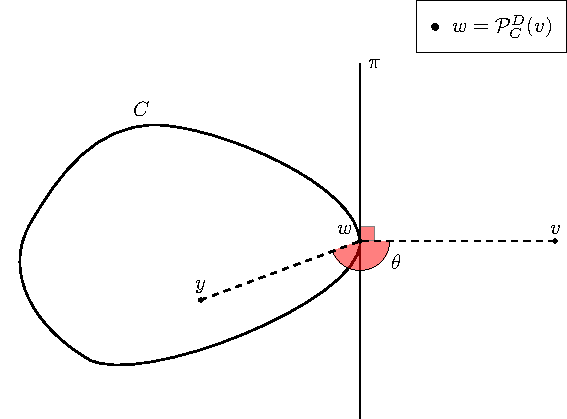
\includegraphics{figures/exactProj.pdf}
	\caption{Exact projection of the point $v$ onto $C$.}
	\label{fig:exactProj}
\end{figure}


\begin{remark}\normalfont \label{re:cproj}
	It follows from Lemma~\ref{pr:cham}  that $\|{\cal P}_{C}^{D}(v)-{\cal P}_{C}^{D}(u)\|_{D}\leq \|v-u\|_{D}$.  Moreover, since   $D\in {\cal D}_{\mu}$, by \eqref{eq:pnv}, we conclude that   ${\cal P}_{C}^{D}(\cdot)$ is Lipschitz continuous with constant $L=\mu$.   Furthermore,  if  $(D_k)_{k\in\mathbb{N}}\subset {\cal D}_{\mu}$,    $\lim_{k\to +\infty} z^{k} = \bar{z}$, and   $\lim_{k \to +\infty} D_{k} = \bar{D}$, then $\lim_{k \to +\infty}{\cal P}_{C}^{D_k}(z^{k})= {\cal P}_{C}^{\bar D}(\bar{z})$, see   \cite[Proposition~4.2]{CombettesVu2013}.
\end{remark}\

\section{The first feasible inexact projection}

In the following, we recall  the  concept of a  feasible inexact projection with respect to $\| \cdot \| _{D}$ relative to a fixed point.

\begin{definition} \label{def:InexactM}
	The {\it feasible inexact projection mapping, with respect to the norm $\| \cdot \|_{D}$,   onto $C$}  relative to a point  $u \in C$ and forcing parameter $\zeta\in (0, 1]$, denoted by ${\cal P}_{C,\zeta}^{D}(u,  \cdot): {\mathbb R}^n \rightrightarrows C$,  is the set-valued mapping defined as follows
	\begin{equation} \label{eq:Projwm}
		{\cal P}_{C,\zeta}^{D}(u, v) := \left\{w\in C:~ \|w-v\|_{D}^2\leq \zeta \| {\cal P}_{C}^{D}(v)-v\|_{D}^2+(1-\zeta)\|u-v\|_{D}^2 \right\}.
	\end{equation}
	Each point $w\in {\cal P}_{C,\zeta}^{D}(u, v) $ is called a  feasible inexact projection,  with respect to the norm $\| \cdot \|_{D}$,  of $v$ onto $C$ relative to $u$ and forcing parameter $\zeta\in (0, 1]$.
\end{definition}
	\begin{remark}\normalfont
		It follows from Definition~\ref{def:InexactM} that ${\cal P}_{C,\zeta}^{D}(u, v)$ is a set generated by the intersection of $C$ and a sphere centered in $v$ and radius given by
		$$
			\zeta \| {\cal P}_{C}^{D}(v)-v\|_{D}^2+(1-\zeta)\|u-v\|_{D}^2.
		$$
		If $\zeta = 1$, then ${\cal P}_{C,1}^{D}(u, v) = \{{\cal P}_{C}^{D}(v)\}$ is the exact projection of $v$ onto $C$. However, when $\zeta$ is close to zero, the radius of sphere is close to $\|u-v\|_{D}$. The inexact condition appears when we consider points that do not minimize the distance from $C$ to $v$, contrary to property \eqref{eq:exactM}. This situation is illustrated in Figure~\ref{fig:martinezProj}.
	\end{remark}\normalfont

\begin{figure}[H]
	\centering
	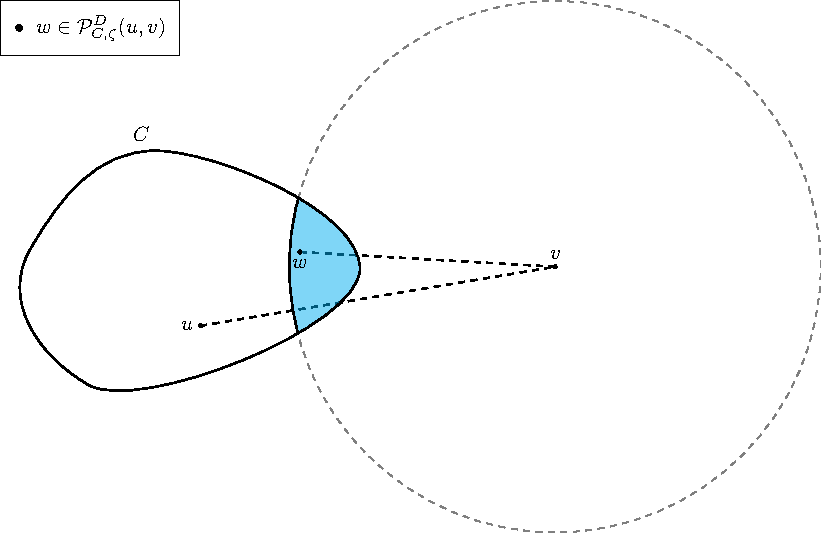
\includegraphics{figures/martinezProj.pdf}
	\caption{Feasible inexact projection of the point $v$ onto $C$.}
	\label{fig:martinezProj}
\end{figure}

In the following, we show that the definition given above is nothing more than a reformulation of the concept of  relative feasible inexact projection with respect to $\| \cdot \|_{D}$  introduced in  \cite{BirginMartinezRaydan2003}.
\begin{remark}\normalfont
	Let $u\in C$, $v\in \mathbb{R}^n$ and  $D$ be   an $n\times n$ positive definite matrix. Consider the quadratic  function $Q: \mathbb{R}^n \to \mathbb{R}$ defined by
	$$
		Q(z):=(1/2) \left\langle {D}(z-u),z-u\right\rangle +  \left \langle D(u-v), z-u \right\rangle.
	$$
	Thus,  letting  $\| \cdot \|_{D}$  be  the norm  defined by \eqref{def:normaD},  some algebraic manipulations   shows that
	\begin{equation} \label{eq:qppq}
		\|z-v\|^2_{D}= 2Q(z) +\|u-v\|^2_{D}.
	\end{equation}
	Hence,  \eqref{eq:qppq}  and \eqref{eq:exactM}  implies  that    ${\cal P}_{C}^{D}(v)=\arg \min _{z\in C}Q(z).$
	Let $\zeta\in (0, 1]$. Thus, by using \eqref{eq:qppq},  after some calculations,  we can see that  the following inexactness condition  introduced in \cite{BirginMartinezRaydan2003},
	$$
		w\in C, \qquad Q(w)\leq \zeta Q ( {\cal P}_{C}^{D}(v)) ,
	$$
	is  equivalent to find  $w\in C$ such that
	$$
		\|w-v\|_{D}^2\leq \zeta \| {\cal P}_{C}^{D}(v)-v\|_{D}^2+(1-\zeta)\|u-v\|_{D}^2,
	$$
	which corresponds to condition \eqref{eq:Projwm} in Definition~\ref{def:InexactM}.
\end{remark}\normalfont
The  concept of  feasible inexact projection  in Definition~\ref{def:InexactM}  provides  more latitude to   the usual  concept  of exact projection \eqref{eq:exactM}.  The next   remark makes  this more precise.
\begin{remark}\normalfont\label{rem: welldef}
	Let $\zeta$ be positive forcing parameter, $C\subset {\mathbb R}^n$ and $u\in C$ be as in Definition~\ref{def:InexactM}.  First of all note that  ${\cal P}_{C}^{D}( v) \in {\cal P}_{C,\zeta}^{D}(u, v)$. Therefore,  ${\cal P}_{C,\zeta}^{D}(u, v)\neq \varnothing$, for all $u\in C$ and $v\in {\mathbb R}^n$. Consequently, the set-valued mapping ${\cal P}_{C,\zeta}^{D}(u,  \cdot)$ as stated in \eqref{eq:Projwm} is well-defined.   Moreover,  for $\zeta=1$, we have ${\cal P}_{C,1}^{D}(u, v)=\{{\cal P}_{C}^{D}(v)\}$.
	In addition, if $\underline{\zeta}$ and $\bar{\zeta}$ are forcing parameters such that $0<\underline{\zeta}\leq \bar{\zeta}\leq 1$, then ${\cal P}_{C,\bar{\zeta}}^{D}(u, v) \subset {\cal P}_{C,\underline{\zeta}}^{D}(u, v)$.
\end{remark}\normalfont
\begin{lemma} \label{pr:condm}
	Let $v \in {\mathbb R}^n$, $u \in C$ and $w\in {\cal P}_{C,\zeta}^{D}(u, v)$. Then,
	$$
		\left\langle D(v-w), y-w\right\rangle \leq  \frac{1}{2} \|w-y\|_{D}^2 +   \frac{1}{2} \left[\zeta \| {\cal P}_{C}^{D}(v)-v\|_{D}^2+(1-\zeta)\|u-v\|_{D}^2 - \|y-v\|_{D}^2\right] ,   \qquad y \in C.
	$$
\end{lemma}
\begin{proof}
	Let  $y \in C$. Since   $  2\langle D(v-w), y-w\rangle = \|w-y\|_{D}^2 + \|w-v\|_{D}^2-\|v-y\|_{D}^2$,  using \eqref{eq:Projwm}  we have
	$2\langle D(v-w), y-w\rangle = \|w-y\|_{D}^2 + \zeta \| {\cal P}_{C}^{D}(v)-v\|_{D}^2+(1-\zeta)\|u-v\|_{D}^2-\|v-y\|_{D}^2$, which is equivalent to  the desired inequality.
\end{proof}

\section{The second feasible inexact projection}

Next, we recall a second  concept of relative  feasible inexact projection onto a closed convex set, see  \cite{Ademir_Orizon_Leandro2020, OrizonFabianaGilson2018}.  The definition  is as follows.
\begin{definition} \label{def:InexactProjC}
	The {\it feasible inexact projection mapping, with respect to the norm $\| \cdot \|_{D}$,  onto $C$} relative to $u \in C$ and forcing parameter $\gamma\geq 0$, denoted by ${\cal R}_{C,\gamma}^{D}(u, \cdot): {\mathbb R}^n \rightrightarrows C$,  is the set-valued mapping defined as follows
	\begin{equation} \label{eq:Projw}
		{\cal R}_{C,\gamma}^{D}(u, v):= \left\{w\in C:~\left\langle D(v-w), y-w \right\rangle \leq \gamma \|w-u\|_{D}^2, \quad \forall~ y \in C \right\}.
	\end{equation}
	Each point $w\in {\cal R}_{C,\gamma}^{D}(u, v)$ is called a feasible inexact projection,  with respect to the norm $\| \cdot \|_{D}$,  of $v$ onto $C$ relative to $u$ and forcing parameter $\gamma\geq 0$.
\end{definition}
The concept of  feasible inexact projection  in Definition~\ref{def:InexactProjC} also  provides  more latitude to  the usual concept  of exact projection. Next,  we present some remarks about this concept.
\begin{remark}\normalfont\label{rem: welldef}
	Let $\gamma\geq 0$ be a forcing parameter, $C\subset {\mathbb R}^n$ and $u\in C$ be as in Definition~\ref{def:InexactProjC}.
	For all $v\in {\mathbb R}^n$, it follows from \eqref{eq:Projw} and Lemma~\ref{pr:cham} that ${\cal R}_{C,0}^{D}(u, v)=\{{\cal P}_{C}^{D}(v)\}$ is the exact projection of $v$ onto $C$. Moreover, ${\cal P}_{C}^{D}(v)\in {\cal R}_{C,\gamma}^{D}(u, v)$ concluding  that ${\cal R}_{C, \gamma}(u, v)\neq \varnothing$, for all $u\in C$ and $v\in {\mathbb R}^n$. Consequently, the set-valued mapping ${\cal R}_{C,\gamma}^{D}(u, \cdot)$ as stated in \eqref{eq:Projw} is well-defined.
\end{remark}\normalfont

We show now a geometric interpretation for the inexact projection defined in Definition~\ref{def:InexactProjC}.
\begin{remark}\normalfont
	Let $C\subset \mathbb{R}^n$, $u\in C$, $v\in \mathbb{R}^n$, $w\in{\cal R}_{C,\gamma}^{D}(u, v)$ be as stated in Definition~\ref{def:InexactProjC} and $w_t = w+t(v-w)$, with $0\leq t <1$. It is easy to see that, for all $y\in C$,
	\begin{align*}
		\begin{aligned}
			% w_t - w & = t(v-w)        \\
			% v-w_t   & = (1-t)(v-w)    \\
			y-w_t   & = y-w - t(v-w).
		\end{aligned}
	\end{align*}
\end{remark}
It follows from \eqref{eq:Projw} that $\left\langle D(v-w), y-w \right\rangle \leq \gamma \|w-u\|_{D}^2$, so we have
\begin{align*}
	\begin{aligned}
		\left\langle D(v-w_t), y-w_t \right\rangle & = (1-t)\left\langle D(v-w), y-w \right\rangle - t(1-t)\|v-w\|_D^{2} \\
		                                           & \leq  (1-t)\left[ \gamma \|w-u\|_D^2 - t\|v-w\|_D^2 \right].
	\end{aligned}
\end{align*}
Since $0\leq t<1$,
$$
	\|w_t-w\|_D^2 = t^2 \|v-w\|_D^2 \leq t\|v-w\|_D^2,
$$
if
\begin{equation}\label{eq:condProj}
	\gamma \|w-u\|_D^2 \leq \|w_t-w\|_D^2
\end{equation}
then $\left\langle D(v-w_t), y-w_t \right\rangle\leq 0$. In this case the inexact condition appears considering that there is $w_t$ between $w$ and $v$ that satisfies \eqref{eq:condProj} and consequently the condition \eqref{eq:exactA}.  This situation is illustrated in Figure~\ref{fig:condProj1}.


\begin{figure}[H]
	%\begin{adjustwidth}{2.2cm}{2.2cm}
	\begin{subfigmatrix}{2}
		\subfigure[Geometric interpretation.]{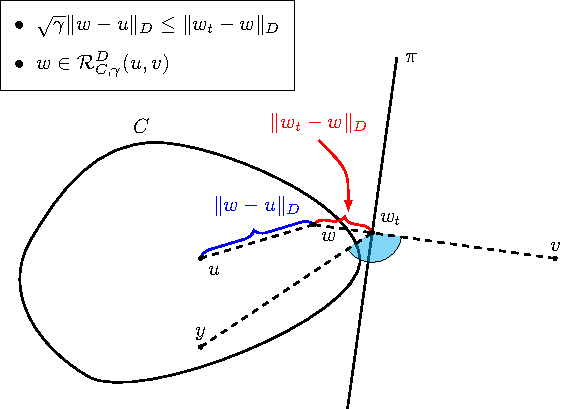
\includegraphics{figures/condProj1.pdf}}
		\subfigure[Example of ${\cal R}_{C,\gamma}^{D}(u, v)$.]{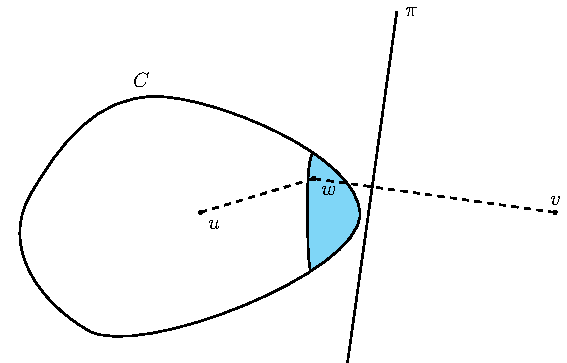
\includegraphics{figures/condProj2.pdf}}
	\end{subfigmatrix}
	\caption{Geometric interpretation of projection ${\cal R}_{C,\gamma}^{D}(u, v)$.}
	\label{fig:condProj1}
	%\end{adjustwidth}
\end{figure}
	In the following we presents some examples of regions given by inexact projection ${\cal R}_{C,\gamma}^{D}(u, v)$. Note that the projection ${\cal R}_{C,\gamma}^{D}(u, v)$ gets smaller as $u$ gets closer to $w$.
\begin{figure}[H]
	%\begin{adjustwidth}{2.2cm}{2.2cm}
	\begin{subfigmatrix}{3}
		\subfigure[]{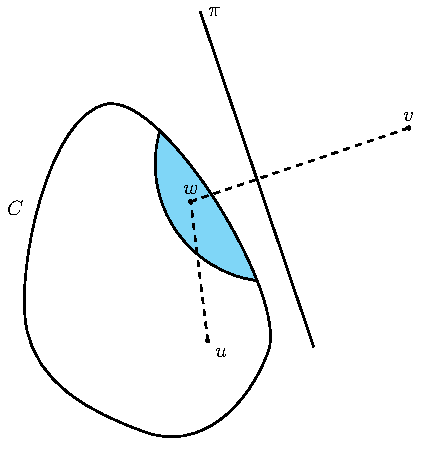
\includegraphics{figures/condProj3.pdf}}
		\subfigure[]{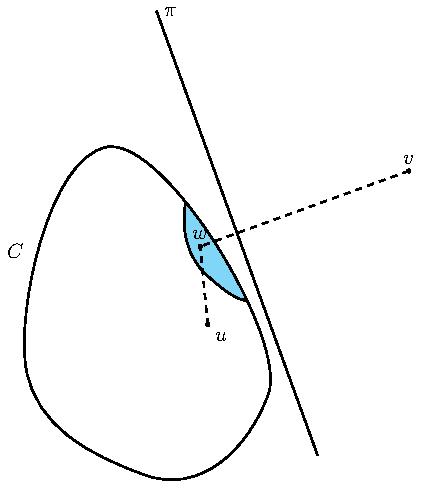
\includegraphics{figures/condProj4.pdf}}
		\subfigure[]{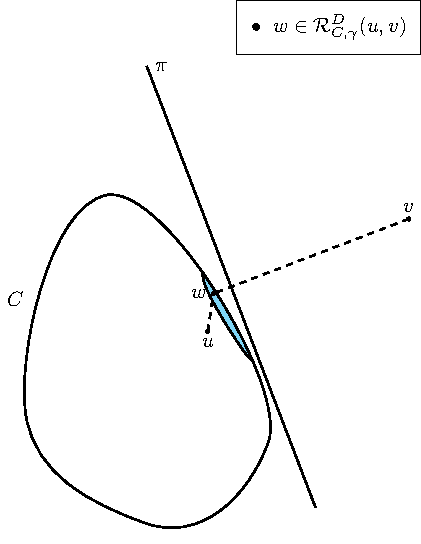
\includegraphics{figures/condProj5.pdf}}
	\end{subfigmatrix}
	\caption{Examples of regions given by inexact projection ${\cal R}_{C,\gamma}^{D}(u, v)$.}
	\label{fig:baseline}
	%\end{adjustwidth}
\end{figure}
The next example shows the behavior of the projection ${\cal R}_{C,\gamma}^{D}(u, v)$ when the set $C$ has a vertice and some flat parts.
\begin{figure}[H]
	%\begin{adjustwidth}{2.2cm}{2.2cm}
	\begin{subfigmatrix}{3}
		\subfigure[]{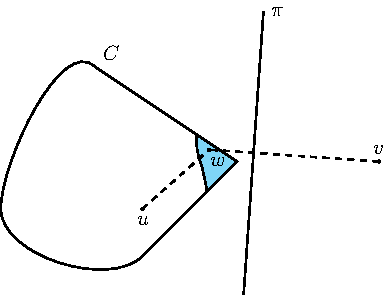
\includegraphics[width=0.3\linewidth]{figures/condProj6.pdf}}
		\subfigure[]{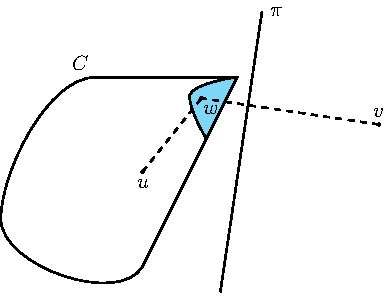
\includegraphics[width=0.3\linewidth]{figures/condProj7.pdf}}
		\subfigure[]{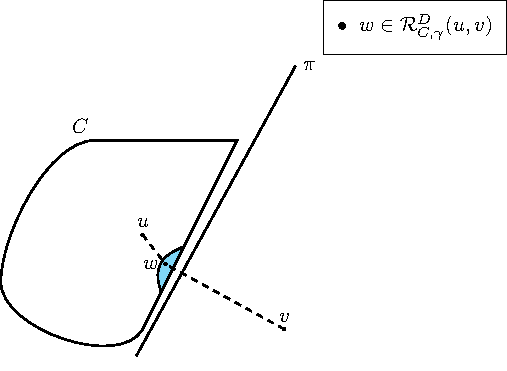
\includegraphics[width=0.38\linewidth]{figures/condProj8.pdf}}
	\end{subfigmatrix}
	\caption{Examples of regions given by inexact projection ${\cal R}_{C,\gamma}^{D}(u, v)$.}
	\label{fig:baseline}
	%\end{adjustwidth}
\end{figure}

The  next lemma is a variation of \cite[Lemma 6]{Reiner_Orizon_Leandro2019}.  It will allow to relate Definitions~\ref{def:InexactM} and \ref{def:InexactProjC}.
\begin{lemma} \label{pr:cond}
	Let $v \in {\mathbb R}^n$, $u \in C$, $\gamma \geq 0$ and $w\in {\cal R}_{C,\gamma}^{D}(u, v)$. Then,  for all $0 \leq \gamma <1/2$, the holds
	$$
		\displaystyle \|w-x\|_{D}^2 \leq \|x-v\|_{D}^2 + \frac{2\gamma}{1-2\gamma}\|u-v\|_{D}^2- \frac{1}{1-2\gamma}\|w-v\|_{D}^2, \qquad \forall x \in C.
	$$
\end{lemma}
\begin{proof}
	First note that $\|w-x\|_{D}^2 = \|x-v\|_{D}^2 - \|w-v\|_{D}^2 + 2 \langle D(v-w), x-w \rangle$. Since $w \in {\cal R}_{C,\gamma}^{D}(u, v)$ and $x \in C$, combining the last equality with \eqref{eq:Projw}, we obtain
	\begin{equation} \label{eq:fg}
		\|w-x\|_{D}^2 \leq \|x-v\|_{D}^2 - \|w-v\|_{D}^2  + 2\gamma \|w-u\|_{D}^2.
	\end{equation}
	On the other hand, we also have $\|w-u\|_{D}^2=\|u-v\|_{D}^2 - \|w-v\|_{D}^2 +  2 \langle D(v-w), u-w \rangle$. Due to $w\in {\cal R}_{C,\gamma}^{D}(u, v)$ and $u \in C$, using \eqref{eq:Projw} and considering that  $0 \leq \gamma < 1/2$, we have
	$$
		\|w-u\|_{D}^2 \leq \frac{1}{1-2\gamma}\|u-v\|_{D}^2 - \frac{1}{1-2\gamma} \|w-v\|_{D}^2.
	$$
	Therefore, substituting the last inequality into   \eqref{eq:fg}, we obtain the  desired inequality.
\end{proof}

\section{The relationship among feasible inexact projections}

In the following  lemma, we present a  relationship between   Definitions~\ref{def:InexactM} and \ref{def:InexactProjC}.
\begin{lemma} \label{pr:condrip}
	Let $v \in {\mathbb R}^n$, $u \in C$, $\gamma \geq 0$  and $\zeta\in (0, 1]$.  If  $0 \leq \gamma <1/2$ and $\zeta=1-2\gamma$, then
	$$
		{\cal R}_{C,\gamma}^{D}(u, v) \subset {\cal P}_{C,\zeta}^{D}(u, v).
	$$
\end{lemma}
\begin{proof}
	Let $w\in {\cal R}_{C,\gamma}^{D}(u, v)$. Applying Lemma~\ref{pr:cond} with  $x={\cal P}_{C}^{D}(v)$ we have
	$$
		\|w-{\cal P}_{C}^{D}(v)\|_{D}^2 \leq \|v-{\cal P}_{C}^{D}(v)\|_{D}^2 + \frac{2\gamma}{1-2\gamma}\|u-v\|_{D}^2- \frac{1}{1-2\gamma}\|w-v\|_{D}^2,
	$$
	After some algebraic manipulations in the last inequality we obtain that
	$$
		\|w-v\|_{D}^2 \leq (1-2\gamma)\|v-{\cal P}_{C}^{D}(v)\|_{D}^2 + 2\gamma\|u-v\|_{D}^2- (1-2\gamma)\|w-{\cal P}_{C}^{D}(v)\|_{D}^2.
	$$
	Therefore, considering that  $0 \leq \gamma <1/2$ and $\zeta=1-2\gamma$, the result follows from Definition~\ref{def:InexactM}.
\end{proof}

\begin{remark}\normalfont \label{re:ni}
	Under the conditions of  Lemma \ref{pr:condrip}, there exists  $0 \leq \gamma <1/2$ and $\zeta=1-2\gamma$ such that ${\cal P}_{C,\zeta}^{D}(u, v)  \nsubseteq    {\cal R}_{C,\gamma}^{D}(u, v)$. Indeed,  let $\gamma=3/8$, $\zeta=1/4$,  and ${\bar w}=\frac{1}{2}({\cal P}_{C}^{D}(v)+u)$, then
	$$
		\displaystyle\|{\bar w}-v\|_D^2=\frac{1}{4}\| {\cal P}_{C}^{D}(v)-v\|_D^2 + \frac{1}{4}\|u-v\|_D^2 +\frac{1}{2} \langle D( {\cal P}_{C}^{D}(v) -v), u-v \rangle.
	$$
	Since  $ {\cal P}_{C}^{D}(v)$ is the exact projection of $v$,  we have   $\displaystyle\langle D( {\cal P}_{C}^{D}(v) -v), u-v \rangle \leq \|u-v\|_D^2$. Combining this inequality with  the last equality and Definition~\ref{def:InexactM}, we conclude that ${\bar w}\in {\cal P}_{C,\zeta}^{D}(u, v)$. Now,  letting $w_t=t{\cal P}_{C}^{D}(v)+ (1-t){\bar w}$  with $0<t<1$, after some algebraic  manipulations  we have
	$$
		\langle D(v-{\bar w}), w_t-{\bar w} \rangle=t\| {\bar w}-u\|_D^2 - \frac{t}{2} \langle D( v- {\cal P}_{C}^{D}(v)) , u-{\cal P}_{C}^{D}(v)  \rangle.
	$$
	Thus, it follows from Lemma~\ref{pr:cham} that $\displaystyle \langle D(v-{\bar w}), w_t-{\bar w} \rangle\geq t\| {\bar w}-u\|_D^2 $.  Hence,  taking  $t>3/8$ we conclude that ${\bar w}\not\in{\cal R}_{C,\gamma}^{D}(u, v)$.  Therefore, considering that ${\bar w}\in {\cal P}_{C,\zeta}^{D}(u, v)$, the statement follows.
\end{remark}\normalfont
It follows from Remark~\ref{re:ni} that, in general,  ${\cal P}_{C,\zeta}^{D}(u, v)  \nsubseteq    {\cal R}_{C,\gamma}^{D}(u, v)$. However, whenever $C$ is a bounded set,  we will show  that   for each  fixed  $0 \leq \gamma <1/2$  there exist $0 < \zeta  <1$ such that    ${\cal P}_{C,\zeta}^{D}(u, v)  \subseteq    {\cal R}_{C,\gamma}^{D}(u, v)$. For that, we first need the next lemma.
\begin{lemma} \label{le:epsi}
	Let $v \in {\mathbb R}^n$, $u \in C$ and $0<\gamma < 1/2$. Assume that $C$ is a bounded set and take
	\begin{equation} \label{eq:epsi}
		0<\varepsilon < \frac{\gamma \|u-\mathcal{P}_C^D(v)\|_D^2}{1-\gamma+\|v-\mathcal{P}_C^D(v)\|_D+ 2	\gamma\|u-\mathcal{P}_C^D(v)\|_D+\mbox{\normalfont diam}C },
	\end{equation}
	where $\mbox{\normalfont diam}C$ denotes the diameter of $C$. Then, $\{w\in C: ~ \|w-\mathcal{P}_C^D(v)\|_D\leq \varepsilon\}\subset\mathcal{R}_{C,\gamma}^D(u, v)\}$.
\end{lemma}
\begin{proof}
	Take $\varepsilon$ satisfying \eqref{eq:epsi} and $w\in C$ such that  $\|w-\mathcal{P}_C^D(v)\|_D\leq \varepsilon$ . For all $z\in C$, we have
	\begin{multline*}
		\langle D(v-w), z-w \rangle = \langle D(v-\mathcal{P}_C^D(v)),z-\mathcal{P}_C^D(v) \rangle + \langle D(v-\mathcal{P}_C^D(v)), \mathcal{P}_C^D(v) -w \rangle\\
		+ \langle D(\mathcal{P}_C^D(v) - w), z- \mathcal{P}_C^D(v) \rangle +\| \mathcal{P}_C^D(v)-w\|_D^2.
	\end{multline*}
	Using Lemma~\ref{pr:cham},  we have $\langle D(v-\mathcal{P}_C^D(v)),z-\mathcal{P}_C^D(v) \rangle\leq 0$. Thus, the last equality becomes
	$$
		\langle D(v-w), z-w \rangle \leq \langle D(v-\mathcal{P}_C^D(v)), \mathcal{P}_C^D(v) -w \rangle + \langle D(\mathcal{P}_C^D(v) - w), z- \mathcal{P}_C^D(v) \rangle +\| \mathcal{P}_C^D(v)-w\|_D^2.
	$$
	By using Cauchy-Schwarz inequality, we conclude from the last inequality that
	$$
		\langle D(v-w), z-w \rangle \leq  \|w-\mathcal{P}_C^D(v) \|_D\left(\|v-\mathcal{P}_C^D(v)\|_D+ \|z- \mathcal{P}_C^D(v)\|_D\right) +\|w-\mathcal{P}_C^D(v)\|_D^2.
	$$
	Since $\|w-\mathcal{P}_C^D(v)|_D\leq \varepsilon$ and $ \|z- \mathcal{P}_C^D(v)\|_D\leq \mbox{diam} C$, the last inequality implies that
	\begin{equation}\label{eq:diam1}
		\langle D(v-w), z-w \rangle \leq \varepsilon \left(\|v-\mathcal{P}_C^D(v)\|_D+\mbox{diam}C\right)+\varepsilon^2,
	\end{equation}
	On the other hand, if $\varepsilon$ satisfies \eqref{eq:epsi} then
	$$
		\varepsilon \left( 1-\gamma+\|v-\mathcal{P}_C^D(v)\|_D+ \mbox{diam} C\right) + \gamma \varepsilon^2 <
		\gamma\|u-\mathcal{P}_C^D(v)\|_D^2-2	\gamma\varepsilon\|u-\mathcal{P}_C^D(v)\|_D +\gamma\varepsilon^2,
	$$
	hence
	$
		\varepsilon \left( 1-\gamma+\|v-\mathcal{P}_C^D(v)\|_D+ \mbox{diam} C\right) + \gamma \varepsilon^2 < \gamma\left(\|u-\mathcal{P}_C^D(v)\|_D-\varepsilon\right)^2.
	$
	Since $\gamma, \varepsilon<1$, we have  $\varepsilon^2 < \varepsilon(1-\gamma) + \gamma \varepsilon^2$ and we can conclude that
	$$
		\varepsilon \left( \|v-\mathcal{P}_C^D(v)\|_D+ \mbox{diam} C\right) + \varepsilon^2 <
		\gamma\left(\|u-\mathcal{P}_C^D(v)\|_D-\varepsilon\right)^2.
	$$
	It follows from \eqref{eq:diam1} that
	\begin{equation}\label{eq:diam2}
		\langle D(v-w), z-w \rangle \leq \gamma\left(\|u-\mathcal{P}_C^D(v)\|_D-\varepsilon\right)^2.
	\end{equation}
	Using again that $\|w-\mathcal{P}_C^D(v)|_D\leq \varepsilon$ and the triangular inequality, we have
	$$
		0<\|u-\mathcal{P}_C^D(v)\|_D -\varepsilon \leq \|u-\mathcal{P}_C^D(v)\|_D -\|w-\mathcal{P}_C^D(v)\|_D \leq \|u-w\|_D.
	$$
	Hence,   taking into account  \eqref{eq:diam2}, we conclude that $	\langle D(v-w), z-w \rangle \leq \gamma\|u-w\|_D^2$. Therefore, it follows from Definition~\ref{def:InexactProjC} that    $w\in\mathcal{R}_{C,\gamma}^D(u, v)$.
\end{proof}
\begin{proposition} \label{le:pcr}
	Let $v \in {\mathbb R}^n$, $u \in C$ and assume that $C$ is a bounded set. Then, for each $0<\gamma < 1/2$,     there exist $0 < \zeta  <1$ such that    ${\cal P}_{C,\zeta}^{D}(u, v)  \subseteq    {\cal R}_{C,\gamma}^{D}(u, v)$.
\end{proposition}
\begin{proof}
	It follows from Lemma~ \ref{le:epsi}  that given $0<\gamma<1/2$ there exists $\varepsilon>0$ such that,  for all $w\in C$  with $\|w-\mathcal{P}_C^D(v)\|\leq \varepsilon$, we have  $w\in\mathcal{R}_\gamma^D(v)$. Otherwise,  we can see in (\ref{eq:Projwm}), when $\zeta\to 1$, the diameter of $C\cap{\cal P}_{C,\zeta}^{D}(u, v)$ tends to zero, then there exists  $\zeta$ close to 1 such that $\mbox{diam}(C\cap{\cal P}_{C,\zeta}^{D}(u, v))<\varepsilon/2$, and ${\cal P}_{C,\zeta}^{D}(u, v) \subset {\cal R}_{C,\gamma}^{D}(u, v)$.
\end{proof}

Next, we present  important properties of  inexact projections,  it  will be useful in  the sequel.
\begin{lemma} \label{Le:ProjProperty}
	Let $x \in C$, $\alpha > 0$ and  $z(\alpha) = x-\alpha D^{-1} \nabla f(x)$. Take $w(\alpha) \in  {\cal P}_{C,\zeta}^{D}(x, z(\alpha))$ with $\zeta\in (0, 1]$. Then,
	\begin{itemize}
		\item[(i)] $\displaystyle \langle \nabla f(x), w(\alpha) - x\rangle \leq -\frac{1}{2\alpha} \|w(\alpha) -x\|_{D}^2 +   \frac{\zeta}{2\alpha} \left[\| {\cal P}_{C}^{D}(z(\alpha))-z(\alpha)\|_{D}^2 - \|x-z(\alpha)\|_{D}^2\right]$;
		\item[(ii)] the point $x$ is stationary for problem \eqref{eq:OptP} if and only if $x \in {\cal P}_{C,\zeta}^{D}(x, z(\alpha))$;
		\item[(iii)] if  $x \in C$ is a nonstationary point for problem \eqref{eq:OptP}, then $\Big\langle \nabla f(x), w(\alpha) - x \Big\rangle < 0$. Equivalently, if there exists ${\bar \alpha}>0$ such that $\Big\langle \nabla f(x), w({\bar \alpha}) - x \Big\rangle \geq 0$, then $x$ is stationary for problem \eqref{eq:OptP}.
	\end{itemize}
\end{lemma}
\begin{proof}
	Since $w(\alpha) \in  {\cal P}_{C,\zeta}^{D}(x, z(\alpha))$, applying Lemma~\ref{pr:condm} with   $w=w(\alpha)$, $v=z(\alpha)$, $y=x$,  and $u=x$, we conclude,  after some algebraic manipulations,  that
	$$
		\left\langle D(z(\alpha)-w(\alpha)), x-w(\alpha) \right\rangle \leq 	\frac{1}{2} \|w(\alpha) -x\|_{D}^2 +   \frac{\zeta}{2} \left[\| {\cal P}_{C}^{D}(z(\alpha))-z(\alpha)\|_{D}^2 - \|x-z(\alpha)\|_{D}^2\right].
	$$
	Substituting  $z(\alpha) = x-\alpha \nabla f(x)$ in the left hand side of the last inequality,   some manipulations yield the inequality of item $(i)$.  For proving item $(ii)$, we first assume that $x$ is stationary for problem \eqref{eq:OptP}. In this case, \eqref{eq:StatPoint} implies that $\langle \nabla f(x), w(\alpha)-x \rangle \geq 0$. Hence,  due to $\|{\cal P}_{C}^{D}(z(\alpha))-z(\alpha)\|_{D}\leq  \|x-z(\alpha)\|_{D}$,   item $(i)$ implies
	$$
		\frac{1}{2\alpha} \|w(\alpha) -x\|_{D}^2 \leq    \frac{\zeta}{2\alpha} \left[\| {\cal P}_{C}^{D}(z(\alpha))-z(\alpha)\|_{D}^2 - \|x-z(\alpha)\|_{D}^2\right]\leq 0.
	$$
	Since $\alpha > 0$ and  $\zeta\in (0, 1]$, the last inequality  yields  $w(\alpha) = x$.  Therefore, $x \in {\cal P}_{C,\zeta}^{D}(x, z(\alpha))$. Reciprocally, if  $x \in {\cal P}_{C,\zeta}^{D}(x, z(\alpha))$, then Definition~\ref{def:InexactM} implies that
	$$
		\|x-z(\alpha)\|_{D}^2\leq \zeta \| {\cal P}_{C}^{D}(z(\alpha))-z(\alpha)\|_{D}^2+(1-\zeta)\|x-z(\alpha)\|_{D}^2.
	$$
	Hence, $0\leq \zeta\left( \| {\cal P}_{C}^{D}(z(\alpha))-z(\alpha)\|_{D}^2-(\|x-z(\alpha)\|_{D}^2\right)$. Considering that  $\zeta\in (0, 1]$ we have
	$$
		\|x-z(\alpha)\|_{D}\leq\| {\cal P}_{C}^{D}(z(\alpha))-z(\alpha)\|_{D}.
	$$
	Thus, due to  exact projection  with respect to the norm $\| \cdot \| _{D}$   be unique and $z(\alpha) = x-D^{-1} \alpha \nabla f(x)$,   we have    ${\cal P}_{C}^{D}( x-\alpha D^{-1} \nabla f(x))=x$. Hence, $x$ is the  solution of the constrained optimization problem $  \min _{y\in C}  \|y-z(\alpha)\| ^{2}_{D}$,
	which taking into account that  $\alpha > 0$ implies \eqref{eq:StatPoint}. Therefore, $x$ is stationary point for problem \eqref{eq:OptP}. Finally, to prove item $(iii)$, take $x$ a nonstationary point for problem \eqref{eq:OptP}. Thus, by item $(ii)$, $x \notin  {\cal P}_{C,\zeta}^{D}(x, z(\alpha))$ and taking into account that $w(\alpha) \in  {\cal P}_{C,\zeta}^{D}(x, z(\alpha))$, we conclude that $x \neq w(\alpha)$. Since $\|{\cal P}_{C}^{D}(z(\alpha))-z(\alpha)\|_{D}\leq  \|x-z(\alpha)\|_{D}$, $\alpha > 0$ and $\zeta\in (0, 1]$, it follows from item $(i)$ that $\Big\langle \nabla f(x), w(\alpha) - x \Big\rangle < 0$ and the first sentence is proved. Finally, note that the second sentence is the contrapositive of the first sentence.
\end{proof}

Finally, it is worth mentioning that Definitions~\ref{def:InexactM} and \ref{def:InexactProjC}, introduced respectively in \cite{BirginMartinezRaydan2003} and \cite{OrizonFabianaGilson2018},  are relative inexact  concepts, while the concept introduced in \cite{SalzoVilla2012,VillaSalzo2013} is absolute.



%%%%%%%%%%%%%%%%%%%%%%%%%%%%%%%%%%
\section{Practical computation of  inexact projections} \label{sec:pcip}

In this section,  for a given  $v\in {\mathbb R}^n$ and   $u \in C$, we discuss how to calculate a  point  $w \in C$ belonging to  ${\cal P}_{C, \zeta}^{D}(u,v)$ or ${\cal R}_{C, \gamma}^{D}(u,v)$.  We recall that  Lemma~\ref{pr:condrip} implies that ${\cal P}_{C, \zeta}^{D}(u,v)$ has  more latitude than ${\cal R}_{C, \gamma}^{D}(u,v)$, i.e., ${\cal R}_{C, \gamma}^{D}(u,v) \subset {\cal P}_{C, \zeta}^{D}(u,v)$.

We begin our discussion by showing how a point $w\in {\cal P}_{C, \zeta}^{D}(u,v)$ can be calculated  without knowing the point ${\cal P}_{C}^{D}(v)$.   Considering that this discussion has already been covered in \cite[Section~3,  Algorithm 3.1]{BirginMartinezRaydan2003},  we will limit ourselves to giving a general idea of how this task is carried out; see also \cite[Section~5.1]{Bonettini2016}.   The idea is to use an external procedure capable of computing two  sequences  $(c_\ell)_{\ell\in\mathbb{N}}\subset \mathbb{R}$  and   $(w^\ell)_{\ell\in\mathbb{N}}\subset C$ satisfying the following  conditions
\begin{equation}\label{def:cl}
	c_\ell \leq \|{\cal P}_{C}^{D}(v)-v\|_D^2,\quad  \forall\ell\in\mathbb{N}, \qquad \qquad \lim_{\ell \to +\infty} c_\ell = \|{\cal P}_{C}^{D}(v)-v\|_D^2, \qquad \quad   \lim_{\ell\to +\infty} w^\ell = {\cal P}_{C}^{D}(v).
\end{equation}
In this case,   if  $v\notin C$, then   we have $ \|{\cal P}_{C}^{D}(v)-v\|_D^2- \|u-v\|_D^2<0$. Hence,   given an arbitrary $ \zeta\in (0,1)$,  the second condition in \eqref{def:cl} implies  that   there exists $\hat{\ell}$ such that
$$
	\|{\cal P}_{C}^{D}(v)-v\|_D^2- \|u-v\|_D^2< \zeta (c_{\hat{\ell}}- \|u-v\|_D^2).
$$
Moreover, by using the last condition in \eqref{def:cl}, we conclude that   there exists $\bar{\ell}>\hat{\ell}$ such that
\begin{equation}\label{def:clsc}
	\|w_{\bar{\ell}}-v\|_D^2- \|u-v\|_D^2< \zeta (c_{\bar{\ell}}- \|u-v\|_D^2),
\end{equation}
which using   the inequality  in \eqref{def:cl} yields  $ \ \|w_{\bar{\ell}}-v\|_D^2<  \zeta \|{\cal P}_{C}^{D}(v)-v\|_D^2  +(1-\zeta) \|u-v\|_D^2$.
Hence, Definition~\ref{def:InexactM} implies that  $w_{\bar{\ell}}\in  {\cal P}_{C, \zeta}^{D}(u, v)$.   Therefore,   \eqref{def:clsc}  can be used as a stopping criterion to compute  a  feasible inexact projection,  with respect to the norm $\| \cdot \|_{D}$,  of $v$ onto $C$ relative to $u$ and forcing parameter $\zeta\in (0, 1]$. For instance,  it follows from   \cite[Theorem~3.2, Lemma~3.1]{BirginMartinezRaydan2003} (see also \cite{BirginRaydan2005}) that  such sequences  $(c_\ell)_{\ell\in\mathbb{N}}\subset \mathbb{R}$  and   $(w^\ell)_{\ell\in\mathbb{N}}\subset C$  satisfying  \eqref{def:cl}  can be computed by using   {\it Dykstra's algorithm} \cite{Dykstra1986, Dykstra1983}, whenever  $D$ is the identity matrix  and the set $C=\cap_{i=1}^p C_i$, where $C_i$ are closed and convex sets and the exact projection  ${\cal P}_{C_i}^{D}(v)$ is easy to obtain, for all $i=1,\dots,p$.

We end this section by discussing how to compute a point $w\in{\cal R}_{C, \gamma}^{D}(u,v)$. For that, we apply the classical {\it Frank-Wolfe method}, also known as {\it conditional gradient method},   to minimize the function  $\psi(z) := \|z - v\|^2/2$ onto  the constraint set $C$ with  a suitable  stop criteria depending  of $u\in C$ and $\gamma \in (0, 1]$, see  \cite{BeckTeboulle2004, Jaggi2013}.  To state the method  we assume the existence of a linear optimization oracle (or simply LO oracle) capable of minimizing linear functions over the constraint set $C$,   which is assumed to be  compact. The   Frank-Wolfe method is  formally stated as follows.

\begin{algorithm}[H]
	\begin{description}
		\item[Input:]  $D\in {\cal D}_{\mu}$,  $\gamma \in (0, 1]$,  $v\in {\mathbb R}^n$ and   $u \in C$.
		\item[ Step 0.] Let $w^0\in  C$ and  set $\ell \gets 0$.
		\item[ Step 1.] Use a LO oracle to compute an optimal solution $z^\ell$ and the optimal value $s_{\ell}^*$ as
			\begin{equation}\label{eq:CondG_{C}}
				z^\ell \in  \arg\min_{z \in  C} \,\langle w^\ell-v, ~z-w^\ell\rangle,  \qquad s_{\ell}^*:=\langle  w^\ell-v, ~z^\ell-w^\ell \rangle.
			\end{equation}
			If $-s^*_{\ell}\leq \gamma \|w^{\ell}-u\|_{D}^2$, then define $w:=w^\ell$ and {\bf stop}.
		\item[ Step 2.]  Compute $\alpha_\ell$ and $w_{\ell+1}$ as
			\begin{equation}\label{eq:step size}
				w_{\ell+1}:=w^\ell+ \alpha_\ell(z^\ell-w^\ell), \qquad {\alpha}_\ell: =\min\left\{1, -s^*_{\ell}/\|z^\ell-w^\ell\|^2 \right\}.
			\end{equation}
			Set $\ell\gets \ell+1$, and go to Step~1.
		\item[Output:]   $w:=w^\ell$.
	\end{description}
	\caption{Frank-Wolfe  method to compute $w\in {\cal R}_{C, \gamma}^{D}(u,v)$}
	\label{Alg:CondG}
\end{algorithm}

Let us  describe the main features of  Algorithm~\ref{Alg:CondG}, i.e.,  the  Frank-Wolfe method applied to the problem $\min_{z \in C}\psi(z)$.   In this case,  \eqref{eq:CondG_{C}} is equivalent to $s_{\ell}^*:=\min_{z \in C}\langle \psi'(w^\ell) ,~z-w^\ell\rangle$. Since $\psi$ is convex, we have $\psi(z)\geq \psi(w^\ell) + \langle \psi'(w^\ell) ,~z-w^\ell\rangle\geq    \psi(w^\ell)  +   s_{\ell}^*$, for all $z\in C$. Define  $ w_*:=\arg \min_{z \in C}\psi(z)$ and  $\psi^*:= \min_{z \in C}\psi(z)$. Letting $z= w_*$ in the last inequality,  we obtain $\psi(w^\ell)\geq \psi^* \geq \psi(w^\ell)  +   s_{\ell}^*$, which implies that $s_{\ell}^*< 0$ whenever $\psi(w^\ell)\neq \psi^*$. Thus, we conclude that  $-s_{\ell}^*=\langle  v-w^\ell, ~z^\ell-w^\ell \rangle>0\geq  \langle  v-w_*, ~z-w_* \rangle$,  for all~$z\in C$.   Therefore, if  Algorithm~\ref{Alg:CondG} computes  $w^\ell \in C$ satisfying $-s_{\ell}^*\leq  \gamma \|w^{\ell}-u\|_{D}^2$, then the method terminates. Otherwise, it computes the step size $\alpha_\ell = \arg\min_{\alpha \in [0,1]} \psi(w^\ell + \alpha(z^\ell - w^\ell))$  using exact minimization.  Since $z^\ell$, $w^\ell \in C$  and $C$ is convex, we conclude from  \eqref{eq:step size}  that $w_{\ell+1} \in C$, thus  Algorithm~\ref{Alg:CondG}  generates a sequence in $C$.  Finally,   \eqref{eq:CondG_{C}} implies that  $\langle  v-w^\ell, ~z-w^\ell\rangle\leq -s_{\ell}^*$, for all  $ z\in C$.  Considering that   \cite[Proposition A.2]{BeckTeboulle2004}  implies that $\lim_{\ell \to +\infty}s_{\ell}^*=0$ and taking into account   the  stopping criteria     $-s_{\ell}^*\leq \gamma \|w^{\ell}-u\|_{D}^2$, we conclude that the output of  Algorithm~\ref{Alg:CondG} is  a feasible inexact projection $w\in {\cal R}_{C, \gamma}^{D}(u,v)$ i.e.,   $\langle  v-w, ~z-w\rangle\leq   \gamma \|w^{\ell}-u\|_{D}^2$, for all $z\in C$.


